%% 11/23/2015
%%%%%%%%%%%%%%%%%%%%%%%%%%%%%%%%%%%%%%%%%%%%%%%%%%%%%%%%%%%%%%%%%%%%%%%%%%%%
% AGUJournalTemplate.tex: this template file is for articles formatted with LaTeX
%
% This file includes commands and instructions
% given in the order necessary to produce a final output that will
% satisfy AGU requirements. 
%
% You may copy this file and give it your
% article name, and enter your text.
%
%%%%%%%%%%%%%%%%%%%%%%%%%%%%%%%%%%%%%%%%%%%%%%%%%%%%%%%%%%%%%%%%%%%%%%%%%%%%
% PLEASE DO NOT USE YOUR OWN MACROS
% DO NOT USE \newcommand, \renewcommand, or \def, etc.
%
% FOR FIGURES, DO NOT USE \psfrag or \subfigure.
% DO NOT USE \psfrag or \subfigure commands.
%%%%%%%%%%%%%%%%%%%%%%%%%%%%%%%%%%%%%%%%%%%%%%%%%%%%%%%%%%%%%%%%%%%%%%%%%%%%
%
% Step 1: Set the \documentclass
%
% There are two options for article format:
%
% 1) PLEASE USE THE DRAFT OPTION TO SUBMIT YOUR PAPERS.
% The draft option produces double spaced output.
% 
% 2) numberline will give you line numbers.

%% To submit your paper:
\documentclass[draft,linenumbers]{agujournal}
\usepackage{siunitx}
\draftfalse

%% For final version.
% \documentclass{agujournal}

% Now, type in the journal name: \journalname{<Journal Name>}

% ie, \journalname{Journal of Geophysical Research}
%% Choose from this list of Journals:
%
% JGR-Atmospheres
% JGR-Biogeosciences
% JGR-Earth Surface
% JGR-Oceans
% JGR-Planets
% JGR-Solid Earth
% JGR-Space Physics
% Global Biochemical Cycles
% Geophysical Research Letters
% Paleoceanography
% Radio Science
% Reviews of Geophysics
% Tectonics
% Space Weather
% Water Resource Research
% Geochemistry, Geophysics, Geosystems
% Journal of Advances in Modeling Earth Systems (JAMES)
% Earth's Future
% Earth and Space Science
%
%

\journalname{<enter journal name here>}


\begin{document}

%% ------------------------------------------------------------------------ %%
%  Title
% 
% (A title should be specific, informative, and brief. Use
% abbreviations only if they are defined in the abstract. Titles that
% start with general keywords then specific terms are optimized in
% searches)
%
%% ------------------------------------------------------------------------ %%

% Example: \title{This is a test title}

\title{Impact of the snow surface on the ice crystal concentration measurements at mountain-top stations}

%% ------------------------------------------------------------------------ %%
%
%  AUTHORS AND AFFILIATIONS
%
%% ------------------------------------------------------------------------ %%

% Authors are individuals who have significantly contributed to the
% research and preparation of the article. Group authors are allowed, if
% each author in the group is separately identified in an appendix.)

% List authors by first name or initial followed by last name and
% separated by commas. Use \affil{} to number affiliations, and
% \thanks{} for author notes.  
% Additional author notes should be indicated with \thanks{} (for
% example, for current addresses). 

% Example: \authors{A. B. Author\affil{1}\thanks{Current address, Antartica}, B. C. Author\affil{2,3}, and D. E.
% Author\affil{3,4}\thanks{Also funded by Monsanto.}}

\authors{Alexander Beck\affil{1}, Jan Henneberger\affil{1}, and Ulrike Lohmann\affil{1}}


% \affiliation{1}{First Affiliation}
% \affiliation{2}{Second Affiliation}
% \affiliation{3}{Third Affiliation}
% \affiliation{4}{Fourth Affiliation}

\affiliation{1}{Institute for Atmospheric and Climate Sciences, ETH Zurich, Zurich, Switzerland}
%(repeat as many times as is necessary)

%% Corresponding Author:
% Corresponding author mailing address and e-mail address:

% (include name and email addresses of the corresponding author.  More
% than one corresponding author is allowed in this LaTeX file and for
% publication; but only one corresponding author is allowed in our
% editorial system.)  

% Example: \correspondingauthor{First and Last Name}{email@address.edu}

\correspondingauthor{Jan Henneberger}{janhenneberger@env.ethz.ch}

%% Keypoints, final entry on title page.

% Example: 
% \begin{keypoints}
% \item	List up to three key points (at least one is required)
% \item	Key Points summarize the main points and conclusions of the article
% \item	Each must be 100 characters or less with no special characters or punctuation 
% \end{keypoints}

%  List up to three key points (at least one is required)
%  Key Points summarize the main points and conclusions of the article
%  Each must be 100 characters or less with no special characters or punctuation 

\begin{keypoints}
\item  In-situ measurements of microphysical cloud properties with a holographic Imager
\item  Influence of in-situ cloud observations at mountain top stations by ground based ice enhancement processes 
\item
\end{keypoints}

%% ------------------------------------------------------------------------ %%
%
%  ABSTRACT
%
% A good abstract will begin with a short description of the problem
% being addressed, briefly describe the new data or analyses, then
% briefly states the main conclusion(s) and how they are supported and
% uncertainties. 
%% ------------------------------------------------------------------------ %%

%% \begin{abstract} starts the second page 

\begin{abstract}
In-situ cloud observations at mountain-top research station regularly measure ice crystal number concentrations (ICNCs) orders of magnitudes higher than expected from measurements of ice nuclei particle concentrations. Several studies suggest that mountain-top in-situ measurements are influenced by surface-based ice-enhancement process, e.g. blowing snow, hoar frost or riming on snow covered trees, rocks and the remaining snow surface. A strong influence of in-situ observations on mountain-top stations by surface-based ice-enhancement processes may limit the relevance of such measurements and could have an impact on orographic clouds.

This study assesses the influence of surface-based ice-enhancement processes on in-situ cloud observations at the Sonnblick Observatory in the Hohen Tauern Region, Austria. Vertical profiles of ICNCc above a snow covered surface were observed up to a height of 10\,\si{m}. A decrease of the ICNC by at least a factor of two is observed, if the maximum ICNC is larger than 100\,\si{l^{-1}}. This decrease can be up to one order of magnitude during in cloud conditions and reached its maximum of more than two orders of magnitudes when the station was not in cloud. On one day a similar decrease of regular and irregular ice crystals was observed with height, which cannot be explained by surface-based ice-crystal enhancement processes. A mechanism is proposed that possibly enhances the ICNC close to the surface when cloud particles sediment and are captured in a turbulent layer above the surface. These observations strongly suggest that mountain-top in-situ measurements poorly represent the true properties of the cloud in contact with the surface. They are influenced not only by surface-based ice-enhancement processes, but possibly also by ICNC enhancement due to turbulent layers above the surface. 
\end{abstract}


\section{Introduction}
The microphysical properties (e.g. phase composition, cloud particle number concentrations) and cloud processes are key parameters for the clouds lifetime, the cloud extent, as well as the intensity of precipitation they produce \citep{Rot07}. For example, the phase composition influences the radiative properties of mid-level clouds in the temperature range between 0 to -35\,\si{^\circ C}. Globally, only pure liquid clouds in this temperature regime reflect 17\,\si{W\,m^{-2}} more radiation back to space than only ice clouds clouds \citep{Loh02}. A good representation of orographic mixed-phase clouds is therefore crucial for accurate weather predictions in alpine terrain and improved climate models. 

In-situ measurements are important to further improve our understanding of microphysical properties and fundamental processes of orographic mixed-phase clouds \citep{Bau10} and are frequently conducted at mountain-top research stations. Despite an improved understanding on the origin of ice crystals from nucleation \citep{Dem15, Bos16a} as well as from secondary ice-multiplication processes \citep{Fie17}, the source of most of the ice crystals observed at mountain-top stations and their impact on the development of the cloud remains an enigma \citep{Loh16}.
 
In-situ observations with aircraft usually observe ICNC on the order of 1-10\,\si{l^{-1}} \citep{Gul01}, whereas at mountain-top research stations (e.g. Elk Mountain, USA or Jungfraujoch, Switzerland) or near the snow surface in the Arctic ICNCs of several hundreds to thousands per liter are frequently reported \citep{Rog87, Lac01, Loy15}. Secondary ice multiplication processes like fragmentation \citep{Ran01} or the Hallett-Mossop process \citep{Hal74} are usually ruled out as the source for the observed ice crystals due to the lack of large ice crystals, respectively large cloud droplets or the wrong temperature range. Instead surface-based ice-enhancement processes are proposed to produce such enormous ICNCs. \citet{Rog87} suggested two possible processes as a source for the observed ICNC: riming on trees, rocks and the snow surface or the lifting of snow particles from the surface, i.e. blowing snow. In addition, \citet{Loy15} suggested hoar frost as a wind independent, surface-based ice-enhancement process to cause ICNCs larger than 100\,\si{l^{-1}} for which they did not observe a wind speed dependency as expected for blowing snow. Although different studies are strife about the mechanisms to explain the measured high ICNCs, they agree on a strong influence by surface-based processes. 

While the influence of mountain-top measurements by surface-based processes nowadays is accepted, the impact of re-suspended ice crystals on the development of supercooled orographic clouds, e.g. a more rapid glaciation and enhanced precipitation, has not been studied extensively \citep{Gee15}. If the proposed surface-based ice-enhancement processes have the potential to impact the development of a cloud depends primarily on the penetration depth of the reseuspended particle into a cloud, i.e. the maximum height above the surface to which the particles get lifted.   

The height dependency of blowing snow has been studied in the context of snow redistribution ("snow drift") and reduced visibility due to the re-suspended ice crystals by observing ice crystals up to several meters above the snow surface \citep{Sch82, Nis05}. It has been reported that blowing snow occurs above a wind speed threshold that varies between 4\,\si{m\,s^{-1}} and 13\,\si{m\,s^{-1}} \citep{Bro88, Li97, Mah03, Der99}. Besides the wind speed, the concentration of blowing snow depends on the snowpack properties (e.g. snow type, time since last snow fall,...) and on the atmospheric conditions (e.g. current temperature, humidity,...) \citep{Vio13}. \citet{Nis05} observed resuspended ice crystals from the surface up to a height of 9.6\,\si{m} and found that the ICNCs usually decrease to as low as 1-10 particles per liter. During a precipitation event, the relative importance of the small ice crystals below < 100\,\si{\mu m} decreases from nearly 100\,\si{\%} at 1.1\,\si{m} to below 20\,\si{\%} at 9.6\,\si{m}. The rapid decrease of ICNCs with height observed in these studies may limit the impact of blowing snow on orographic clouds. However, most of these studies were conducted in dry air conditions where ice crystals undergo rapid sublimation \citep{Yan08}, which may restrict the applicability of these results.

\citet{Loy15} suggested that vapor grown ice crystals on the crystalline surface of the snow cover, i.e. hoar frost, may be detached by mechanical fracturing due to turbulence independent of wind speed. To our knowledge only one modelling study exists, which assesses the impact of haor frost on the development of a cloud. \citet{Far15} implemented a flux of surface hoar crystals in the WRF (Weather Research and Forecasting) model based on a frost flower aerosol flux to simulate ICNCs measured at the Jungfraujoch by \citet{Loy15}. They concluded that the surface-based ice crystals have a limiting impact on orographic clouds because the ice crystals are not advected high into the atmosphere. However, more measurements of ice crystal fluxes from the snow covered surface are necessary to simulate the impact of surface-based ice crystal enhancement processes on the development of orographic clouds \citep{Far15}.

In contrast to these findings, several remote sensing (i.e. satellite, lidar and radar) studies measured ice crystals advected as high as 1\,\si{km} above the surface, which suggests an impact of surface-originated ice crystals on clouds. Satellite observations of blowing snow from MODIS and CALIOP over Antarctica \citep{Pal11} observed layer thickness up to 1\,\si{km} with an average thickness of 120\,\si{m} for all observed blowing snow events. Similar observations from lidar measurements exist from the South Pole with observed layer thicknesses of ice crystals of usually less than 400\,\si{m}, with some rare cases when a subvisual layer exceeded a height of 1\,\si{km} \citep{Mah03}. However, a possible suspension of clear-sky precipitation could not be ruled out as a source of the observed ice crystal layers. Observations of layers of ice crystals from radar measurements on an aircraft in the vicinity of the Medicine Bow Mountains \citep{Val12} observed ground-layer snow clouds which where most of the time not visually detectable but produced a radar signal. Resuspended ice crystals from the surface or riming of cloud droplets at the surface can be the origin of the ice crystals in such ground-layer snow clouds. \citet{Gee15} presented evidence for ice crystals becoming lofted up to 250\,\si{m} in the atmosphere by boundary layer separation behind terrain crests and by hydraulic jumps. Also evidence that ice crystals from the surface may lead to the glaciation of supercooled orographic clouds and enhanced precipitation was found. However, \citet{Gee15} also mentioned the limitation of radar and lidar measurements to separate the small ice crystals produced by surface processes from the larger falling snow particles and more abundant cloud droplets. They even concluded, that "to explore BIP (blowing snow ice particle) lofting into orographic clouds, ice particle imaging devices need to be installed on a tall tower, or on a very steep mountain like the Jungfraujoch".

In this study we assess the influence of surface-based ice-enhancement processes on in-situ cloud observations at mountain-top stations and the potential impact on orographic mixed-phase clouds. Vertical profiles of the ICNC up to a height of 10\,\si{m} above the surface were observed for the first time on a high-altitude mountain station with the holographic imager HOLIMO \citep{Bec17}. HOLIMO is capable of imaging ice crystals larger than 25\,\si{\mu m} and the shape of these ice crystals can be analyzed.

\section{Field Measurements at the Sonnblick Observatory}
\label{sectionMeasurementSite}

\subsection{Site description}

This field campaign was conducted at the Sonnblick Observatory (SBO) situated at the summit of Mt. Sonnblick at 3106\,\si{masl} (\ang{12;57;}E, \ang{47;03;}N) in the Hohen Tauern National Park in the Austrian Alps. The SBO is a meteorological observatory operated all year by the ZAMG (Central Institute for Meteorology and Geodynamics). On the east and south the SBO is surrounded by large glacier fields with a moderate slope, whereas on the northeast a steep wall of approximately 800\,\si{m} descends to the valley (Fig.~\ref{fig:SetUp}, right). Part of the SBO is a 15\,\si{m} high tower used for meteorological measurements by the ZAMG. The data presented in this paper was collected during a field campaign in February 2017. 

\subsection{Instrumentation}
The properties of hydrometeors were observed with the holographic imager HOLIMO, which is part of the HoloGondel platform \citep{Bec17}. The holographic imager was mounted on an elevator that was attached to the meteorological tower of the SBO (Fig.~\ref{fig:Elevator}) to obtain vertical profiles of the hydrometeor properties up to a height of 10\,\si{m} above the surface where the platform was repeatedly positioned at five different heights as indicated in Figure \ref{fig:Elevator}. The holographic imager HOLIMO had a distance of approximately 1.5\,\si{m} from the tower on the east-northeast side of the tower (Fig.~\ref{fig:SetUp}, right). 

The holographic imager HOLIMO yields single particle informations, e.g. size, and shadowgraphs from all cloud particles in a three-dimensional volume on a single image, a so-called hologram. Per hologram, a sample volume of 16\,\si{cm^3} with a length of 6\,\si{cm} along the optical axis is examined. Concentrations and particle size distributions are calculated over 50 holograms corresponding to a volume of 800\,\si{cm^3}. The open source software HoloSuite \citep{Fug15} is used to reconstruct the in-focus images of the particles. Particles smaller than 25\,\si{\um} are classified as liquid droplets, whereas particles larger than 25\,\si{\um} are separated in liquid droplets and ice crystals based on the shape of their 2D image. Similar to a study by \cite{Sch17} the ice crystals were further visually classified into three different groups: regular, irregular and aggregates. Because the visual classification of several thousands of ice crystals is time consuming this sub-classification of ice crystals was done only for the profiles on February 17th.

A single vertical profile was observed within a time interval of 10-12\,\si{min}. By positioning the holographic imager HOLIMO was positioned at an individual height for 2\,\si{min} and recording holograms at 4\,\si{fps}. This results in 8\,\si{l} of sampled air. 
 
%The CIP was located on the north facing side of the measurement terrace of the SBO (see Fig.~\ref{fig:SetUp}, left). Because this location is in the wind shadow of the building of the SBO during south wind cases, the CIP data is only analysed for February 17th, when the wind direction was from North.  

Meteorological data are available from the measurements by the ZAMG. The ZAMG measures one minute averages of temperature, relative humidity and horizontal wind speed and direction at the top of the meteorological tower. Snow cover depth is daily manually observed by the operators of the SBO. Based on these measurements the change of the snow cover is calculated. However, this calculation includes all the changes in the snow cover depth, e.g. snow drift, sublimation, melting and fresh snow. Daily measurements of the total precipitation are available on the north and south side of the SBO. A ceilometer located in the valley north of the SBO measured the cloud base and cloud depth. 

In addition, a 3D sonic anemometer was mounted at the top of the meteorological tower. However, data is only available occasionally, because most of the time the heating of the anemometer was not sufficient to prevent the build up of rime on the measurement arms. 

\section{Results}
\label{Results}

The data presented were observed on 4 February and 17 February, 2017. Figure \ref{fig:meteo0402} and \ref{fig:meteo1702} show an overview on the meteorological conditions on both days. The main difference is the wind direction, which was south-west on 4 February and north on 17 February. 

\subsection{Case study on 4 February, 2017}

On 4 February a low pressure system moved eastwards from the Atlantic Ocean over northern France to western Germany, where it slowly dissipated. Influenced by this low pressure system the wind at the SBO predominantly came from west-southwest and wind speeds were between 10 and 25 \si{m\,s^{-1}} (Fig. \ref{fig:meteo0402}). In the late afternoon, around 1900 UTC, when the low pressure system dissipated over western Germany, the wind direction changed to north and wind speeds decreased to a minimum of 5 \si{m\,s^{-1}}. After 1900 UTC wind speed increased again to up to 15 \si{m\,s^{-1}}. Starting from 0800 UTC the SBO was in cloud except for a short time interval between 1910 and 2020 UTC. Because no data is available from the 3D sonic anemometer, only one minute averages are available from the ZAMG measurements. 

The temperature did not change much during the day and stayed between -10 and -9\,\si{^\circ C} until 1900 UTC when the wind direction changed to north and the temperature decreased to -11\,\si{^\circ C} at 22 UTC.

Between 0830 and 2200 UTC, a total of 24 vertical profiles was obtained, whereas the SBO was in cloud except for a short time period between 1910 and 2020 UTC (blue shaded in Fig. \ref{fig:meteo0402}). The ICNC reached a maximum at 2.5\,\si{m} above the surface (Fig. \ref{fig:Total0402}). Compared to this maximum, the mean ICNC at a height of 10\,\si{m} decreases by a factor of two and the median ICNC even by a factor of four. This strong decreased of ICNC with height suggests that the majority of the ice crystals near the ground originate from the snow surface.

The whole measurement time period on February 4th was divided in four periods representing different conditions (Fig. \ref{fig:profiles0402}). Between 1910 and 2010 UTC (Fig. \ref{fig:profiles0402} third row), when the SBO was not in cloud, the ICNC has its maximum at a height of 2.5\,\si{m}, where it reaches up to 600\,\si{l^{-1}}. For three of the profiles, the ICNC decrease by more than a factor of 5 from over 100\,\si{l^{-1}} at 2.5\,\si{m} to less than 20\,\si{l^{-1}} at 10\,\si{m}. The mean ICNCs decreases from around 100\,\si{l^{-1}} at 2.5\,\si{m} to 10\,\si{l^{-1}} at 10\,\si{m} (Fig. \ref{fig:profiles0402}, right panel in the third row). The large extent of the shaded area at 2.5\,\si{m} represents the high variability of the ICNC even when the data is averaged over 800\,\si{cm^3}. Because the SBO was not in cloud during this time period, these measurements strongly suggest that up to several hundreds of ice crystals per liter originated from surface-based processes at a height of 2.5\,\si{m} and at a wind speed of less than 10\,\si{m\,s^{-1}}. 

Between 2030 and 2200 UTC (Fig. \ref{fig:profiles0402} first row), when the SBO was in cloud again, the vertical profiles of the ICNC show a similar tendency as in the cloud free period. The maximum of the ICNC was observed at a height of 4.1\,\si{m} and the ICNC decreased consistently for all four profiles with height. The mean of the ICNC decreased by a factor of 9 from its maximum at 4.1\,\si{m} to its minimum at 10\,\si{m}. This decrease is on the same order of magnitude as in the cloud free case discussed above. Assuming that the observed ICNC at 10\,\si{m} is representative for the cloud without surface influence, the surface-based processes contribute with several hundreds of ice crystals per liter to the measurements at 2.5, 4.1 and 6.0\,\si{m}. This surface-based contribution is on the same order of magnitude as the total measured ICNCs in the cloud free period observed between 1910 and 2020 UTC. In contrast to the cloud free period, the surface influence now extends to a height of 6.0\,\si{m}, which can be explained by the increased wind speed of up to 15\,\si{m\,s^{-1}}. 

The highest ICNCs were observed in the time period between 1200 and 1500 UTC (Fig. \ref{fig:profiles0402} second row) when also the wind speed reached its maximum of 25\,\si{m\,s^{-1}}. The boxplot shows a maximum ICNC at 2.5\,\si{m} in the range of 500 to 900\,\si{l^{-1}} and a decrease by a factor of 2 within 7.5\,\si{m}. This decrease is much lower than observed in the previous time interval and is most likely due to the high wind speeds. Between different profiles the ICNC changed by a factor of ???, however, consistently for all profiles a decreasing ICNC was observed with height.

In the morning between 8300 and 1100 UTC the observed ICNCs (Fig. \ref{fig:profiles0402} first row) are much lower than between 1200 and 1500 UTC, although wind speeds were as high as 20\,\si{m\,s^{-1}}. A possible reason is that the last snow fall was observed 3 days before the measurements. During these time, the loose ice crystals at the surface where blown away and the snowpack was solidified by temporal melting and re-freezing of the snowpack. Consequently, higher wind speeds are necessary to re-suspend ice crystals from the snowpack. 

The correlation between wind speed and ICNC for 1\,\si{min} time intervals is shown in Figure \ref{fig:ICNCvsWSMAX0402}. The maximum wind speeds is used rather the average wind speed, because it is expected that the gusts, i.e. the highest wind speed in a time interval are most relevant for resuspending ice crystals from the surface. For the time interval between 0830 and 1500 UTC when the wind direction was west-southwest no correlation is observed with wind speeds higher than 14\,\si{m\,s^{-1}} (Fig \ref{fig:ICNCvsWSMAX0402}, top). For the time interval between 1910 and 2230 UTC, when the wind direction was north, a much more pronounced dependency of the ICNC on wind speed is observed for wind speeds lower than 14\,\si{m\,s^{-1}} (Fig \ref{fig:ICNCvsWSMAX0402}, bottom). ICNCs reached a saturation for wind speed larger than 14\,\si{m\,s^{-1}}.

\subsection{17 February 2017}
On 17 February a cold front over northern Europe was moving southwards causing mainly northerly flow across the Alps and at the SBO (Fig. \ref{fig:meteo1702}). Wind speeds observed at the SBO in the time interval between 1800 and 2000 UTC were between 5 and 10\,\si{m\,s^{-1}} . In the same time interval temperature decreased by 1\,\si{K} from -12.5 to -13.5\,\si{^\circ C}. The SBO was in cloud starting from 1300 UTC with varying visibility between several meters up to several hundreds of meters. Some snow fall was observed in the afternoon between 1300 and 1500 UTC. 

For this day, wind data of the 3D Sonic Anemometer are available, which allow a more detailed analysis of the correlation between the observed ICNC and wind speed. Unfortunately, only four vertical profiles were obtained  due to hardware problems with the computer. The first profile was measured in the morning at 1200 UTC when the SBO was not in cloud and no ice crystals were observed. Three more profiles were observed in the late afternoon starting from 1800 UTC. For these profiles the ice crystals have been classified by hand and subclassified in the three categories: regular, irregular and aggregates.

The three profiles observed in the late afternoon of 17 February showed ICNCs of several hundreds in the lowest height intervals with a maximum between 4.1 and 6.0\,\si{m} (Fig. \ref{fig:profiles1702}). The minimum ICNC was consistently observed for all profiles at 10\,\si{m} and was always below 150\,\si{l^{-1}}. The decrease of the ICNC with height varies between a factor of 2 and 4. In general the observed profiles on this day are similar to the ones observed on 4 February between 2030 and 2200 UTC when similar meteorological conditions were present. Wind direction was mainly north to northeast and wind speed varied between 5 and 10 \,\si{m\,s^{-1}} in both measurement intervals. Only temperature was slightly lower on 17 February.

In contrast to the data of 4 February, no correlation between ICNCs and the horizontal wind speed is observed (Fig. \ref{fig:ICNCvsWind1702}). This holds true for the one minute averages and maximum wind speeds observed by the SBO as well as the one second averages observed with the 3D sonic anemometer. However, ICNC increased with the vertical wind speed. 

All the ice crystals observed on 17 February were classified by hand into aggregates, irregular and regular ice crystals (Fig. \ref{fig:profilesHabits1702}). ICNCs are dominantly irregular ice crystals, which is in good agreement with various other observations (citations). However, it is surprising that the fraction of irregular ice crystals stays constant with height or even increases (Fig. \ref{fig:profilesHabits1702} right panels). Surface-based ice crystal enhancement processes are expected to produce irregular ice crystals. With increasing height this influence is expected to decrease and regular ice crystals are expected to become more important. However, from this data a proportional decrease of the absolute number of regular and irregular ice crystals is observed and is in contradiction to the expectations from surface-based ice-crystal enhancement processes. A further discussion of there results will follow in section \ref{Discussion_comp}. The wind speed dependency of irregular and regular ice ICNCs is comparable, and both increase by a factor of 2 when the vertical wind speed increases from 0-2\,\si{m\,s^{-1}} to 4-6\,\si{m\,s^{-1}} (Fig. \ref{fig:ICNCvsWindHabits1702}). Whereas the shape of the size distribution of the irregular ice crystals does not vary much with height, larger regular ice crystals are more strongly reduced with height than smaller regular ice crystals (Fig. \ref{fig:spectrum17}). 



\section{Discussion}
\label{Discussion}

\subsection{Comparison with the properties of blowing snow observed in the Arctic}
\label{Discussion_comp} 
To better understand if the observed ice crystals are re-suspended from the surface, the results of 17 February, 2017 are compared to the properties of blowing snow observed in the Arctic (\citep{Nis05}) and further discussed. 

It is expected that the majority of the ice crystals re-supsended from the surface has irregular habits, whereas regular ice crystals originated in cloud. Furthermore, for the re-suspended ice crystals a decrease of ICNC is expected with height, with a stronger decrease of the larger ice crystals. This results in a shift of the size distribution to smaller sizes or a decrease of the mean particle diameter with height, as it was also observed by \citet{Nis05}. However, the strongest decrease of the size of the ice crystals was observed below 1\,\si{m} above the snow surface, whereas the size of the ice crystals stayed fairly constant in the range of 70-100\,\si{\mu m} between 1 and 9.6\,\si{m} above ground. It is important to notice that \citet{Nis05} measured the properties of blowing snow above a flat surface in dry air. Sublimation of ice crystals in such an environment additionally reduces the ice crystal diameter. 

%Why do you use a fit?
%Move this paragapah to appendix?
For a better comparison a two-parameter gamma probability density function (gamma-pdf) \citep{Bud66, Sch82} 

\begin{linenomath*}
\begin{equation}
f(\text{d}) = \frac{\text{d}^{\alpha - 1}}{\beta^{\alpha} \Gamma\left(\alpha\right)}\exp\left(-\frac{\beta}{\text{d}}\right) 
\end{equation}
\end{linenomath*}

with the particle diameter \textit{d}, the shape parameter $\alpha$ and the scale parameter $\beta$ is fitted to the results of 17 February for both regular and irregular ice crystals (Fig. \ref{fig:gammaPDF}). The resulting shape parameter $\alpha$ and the mean diameter, represented by the product of the shape and scale parameter of the gamma-pdf, are plotted in Figure \ref{fig:shapeFactor}. 

The mean diameter for both the irregular and regular ice crystals is in the range of the properties of blowing snow, with a decrease from 120 to 70\,\si{\mu m} for regular ice crystals and a rather constant  mean diameter of 100\,\si{\mu m}  for irregular ice crystals (Figure \ref{fig:shapeFactor} left). \citet{Nis05} observed a strong increase of the shape factor from 3 to 10 between 1 and 9.6\,\si{m}. Whereas the shape parameter obtained for the regular ice crystals increases with height, it stays constant for the irregular ice crystals. Most important a decrease of the ICNC for both the irregular and regular ice crystals by a factor of 2 is observed within a height interval of 7.5\,\si{m} (Fig. \ref{fig:profiles1702}). All these findings suggest that the majority of the irregular as well as the regular ice crystals are re-suspended from the snow surface. However, this contradicts our assumptions that the majority of the regular ice crystals originate in cloud and only irregular ice crystals are re-suspended from the surface, as it is observed between 1910 and 2000 UTC on 4 February. Here an inspection of the ice crystal habits by eye showed almost exclusively irregular crystals and therefore this is considered a blowing snow event. As a consequence, either our assumptions are wrong and also regular ice crystals contribute to the ICNC of re-suspended particles or a different mechanism has to be responsible for the enriched ICNC close to the snow surface (Fig. \ref{fig:profilesHabits1702}). 

During the measurements on 17 February the SOB was in cloud. Ice crystals of irregular and regular habits from the cloud sediment and may be kept floating near the surface due to turbulence, which is also responsible for the re-suspension of ice crystals from the surface. However, in this case the sedimenting particles may have never reached the surface and maintained their habit. Such an effect may also enrich ice crystals observed close to the surface, but in this case a snow covered surface is not necessary and the wind threshold is much lower than for surface-based ice crystal enhancement processes, because ice crystals do not have to be detached from the surface. This can explain the observation of high ICNCs on 17 February, where the wind speed was in most cases close to the lower threshold wind speed observed for blowing snow, which is 4\,\si{m\,s^{-1}} \citep{Bro88, Li97, Mah03, Der99}. The result of such a mechanism is a rather constant ICNC above the surface and a similar decrease of the ICNC of regular and regular ice crystals with height, as it was observed on 17 February. 

Although it is proposed that the ICNC is dominated by a mechanism just described, blowing snow still contributes to the ICNC at certain time intervals. During one profile  (Fig. \ref{fig:profilesHabits1702}, top row) the ICNC decreases for irregular and regular ice crystals with one exception for the irregular ice crystals at a height of 6\,\si{m}. Whereas the vertical wind speed during this profile was similar for all heights at 4\,\si{m\,s^{-1}}, it reached a maximum of 5.5\,\si{m\,s^{-1}} when the elevator was positioned at 6\,\si{m}, corresponding to the increased ICNC of the irregular ice crystals. The concentration of regular ice crystals was not affected. This suggests that ice crystals re-suspended from the surface have reached the height of 6\,\si{m} during higher wind speeds and had dominantly irregular habits. 
%I can not follow your explanation and where I can see it in the graph

The difference in the height dependence of the size distribution of regular and irregular ice crystals remains unexplained. Whereas the irregular ice crystals show a constant decrease of the ICNC at all sizes, the size distribution for regular ice crystals is shifted to smaller sizes with increasing height. A possible reason for the decrease of the mean diameter of the regular ice crystals is that the particles in the turbulent layer above the surface grow due to vapor diffusion before they final fall out. Therefore regular ice crystals closer to the surface are larger than the regular ice crystals in cloud. The shift of the size distribution is then caused by smaller ice crystals that just sediment and have not been captured in the turbulent layer. The smaller ice crystals become more important with height and start to dominate the size distribution.


\subsection{Wind dependence of the observed ICNCs}

The observations on 4 February and 17 February show a different correlation of the ICNC with wind speed. The ICNCs observed on 4 February show a dependence only for horizontal wind speeds below 14\,\si{m\,{s^{-1}}} (Fig. \ref{fig:ICNCvsWind1702}), whereas for horizontal wind speeds larger than 14\,\si{m\,s^{-1}} this correlation is not observed probably due to a saturation of blowing snow. On 17 February a correlation is only observed with vertical wind speed available from the 3D sonic anemometer (Fig. \ref{fig:ICNCvsWind1702}). Possibly, the vertical wind speed is a better approximation for the turbulence responsible for the re-suspension of ice crystals from the surface as it was already suggested by \citet{Ham14}. In addition vertical wind speeds play an important role especially at research stations like the SBO and the High Altitude Research Station Jungfraujoch, Switzerland, because ice crystals could nucleate on suitable INP and/or be transported from below the research station to the measurement point. For example \citep{Loy15} observed a dependence on horizontal wind speeds only for ICNCs smaller than 100\,\si{\mu m}, whereas larger ICNCs did not show a dependence on horizontal wind speed. Blowing snow, respectively hoar frost, was proposed as the underlying mechanisms for these observations. We suggest that the larger ice crystals observed by \citet{Loy15} have been transported for a longer time and grown to larger sizes. In this case the vertical wind speed could be more relevant, because the particles may have been transported from below the research station by vertical winds.

It has to be mentioned that various difficulties exist when it comes to observing the correlation between wind speed and ICNCs. Firstly, ICNCs are usually compared to a simultaneously measured wind speed. However, the observed ice crystals have been re-suspended some time before the measurement and transported in the air for some time. In this case the simultaneously observed wind speed is not necessarily the driving force of the process of particle lifting, because ice crystals that were re-suspended from the surface by strong turbulence can be transported higher in the atmosphere by much smaller wind speeds (blowing snow paper). Secondly, wind and ICNC measurements may be performed at two different locations. Especially at mountain-top research station with its many structures, local turbulence responsible for the re-suspension of the observed ice crystals may be not well represented by such a wind measurement. This is also true for this study, where the wind measurement was located on a 15\,\si{m} high meteorological tower. Thirdly, the resuspended ICNC does not only depend on wind speed, but also on age of the snow cover and atmospheric conditions and a possible correlation may be suppressed in a data set with different snowpack and atmospheric conditions. Between 1900 and 2030 UTC on 4 February a decrease of the ICNC was observed with time at a height of 2.5\,\si{m}, possibly because the very loose ice crystals on top of the snow cover were blown away.

Another crucial point for correlating observed ICNCs to wind speed is the averaging time of the data. If the averaging time is small, e.g. 1\,\si{min} it is assumed that the observed ice crystals were re-suspended close to the measurement point and immediately transported. If the averaging time is very large, the effect of blowing snow may be averaged out. In this study we chose an average time of 10-15\,\si{s}. This assumes that the particles were re-suspended at most 50-100\,\si{m} upwind from the measurement point and it is believed that also peaks of large concentrations are not yet averaged out. 


\subsection{Influence of ICNC measurements by a snow surface at mountain-top stations and its impact on clouds}

The results obtained in this study suggest a strong enhancement of the ICNC measured close to the snow surface at mountain-top research stations. On 4 February a blowing snow event was observed when the SBO was not in cloud and the ICNC was enhanced by a factor of 100 at a height of 2.5\,\si{m} when compared to upper levels of the elevator (Fig. \ref{fig:profiles0402}, second row). When the SBO was in cloud an enhancement by a factor of 2-10 was observed in the same height interval. On 17 February a similar decrease of the ICNC was observed for irregular and regular ice crystals. This is in contrast to the expectations for blowing snow and a different mechanism is proposed, which enhances the ICNC close to the surface when sedimenting ice crystals are captured in turbulence. The observed ICNC close to the surface is also at least 2 times larger than at a height of 10\,\si{m}. Therefore, we propose that measurements of the ICNC close to the surface do not represent real cloud properties. 

An estimation of the influence of cloud properties by re-suspended ice crystals is difficult, because of the limited vertical extent of the profiles obtained in this study. For most of the profiles the ICNC still shows a decreasing tendency at a height of 8-10\,\si{m} and a final statement of the in-cloud ICNC is not possible. Only for the profiles after 1900 UTC a constant ICNC is observed for the upper levels of the elevator (Fig. \ref{fig:profiles0402}, two bottom rows). From the observation between  2030 and 2200 UTC, when the SOB was in cloud, the in-cloud ICNC can be estimated, when the observed ICNC during the blowing snow event between 1900 and 2000 UTC is subtracted for the upper levels of the elevator. This results in a ICNC of several tens per liter. Between 1200 and 1500 UTC (Fig. \ref{fig:profiles0402}, second row) the wind speed was much higher and the influence of blowing snow possibly extended much higher up in the atmosphere. Because the number of ice nucleating particles in clouds is on the order of 1-10\,\si{l^{-1}}, already ice crystals of the same concentration re-suspended from the surface and lifted high up into the cloud can have a significant impact on the clouds properties, e.g. extent and lifetime. 

To better understand the mechanisms that are responsible for an enhanced ICNC close to the surface and to further investigate the mechanisms proposed in this study we suggest a more thorough field campaigned with additional 3D sonic anemometers at the surface to capture turbulence that may be responsible for the re-supsension of ice crystals, a second 3D sonic anemometer on the elevator and a third 3D anemometer on the top of the tower. This may help to better understand the wind dependence of the ICNC and to find the origin of the observed ice crystals. At best at three cloud imaging probes are part of such a campaign and installed parallel to the 3D sonic anemometer. In addition, to get a better estimate of the impact of re-suspended particle on cloud porperties, especially for high wind speeds, the vertical profiles have to be extended to larger heights above the surface. Such a field campaign could be conducted using a tethered balloon system equipped with cloud imaging probes, which can be lifted several hundreds of meters into the atmosphere.

\section{Conclusion \& Outlook}
This study assessed the influence of mountain-top in-situ measurements by surface-based ice-crystal sources and possible implications on atmospheric relevance of such measurements. An elevator was attached to the meteorological tower of the SBO, Austria and vertical profiles of the ICNC were observed with the holographic imager HOLIMO on two days in February 2017. The main findings are:

\begin{itemize}
\item ICNCs decrease with height. ICNCs near the ground are at least a factor of two larger than at a height of 10\,\si{m} (if the ICNC near the ground is larger than 100\,\si{l^{-1}}). The increase in ICNCs near the ground can be up to an order of magnitude during cloud events and even two magnitudes during cloud free periods. Therefore, in-situ measurements of the ICNC at mountain-top research stations close to the surface overestimate the ICNC.
\item On 4 February ICNCs show a dependence on wind speed for wind speeds up to 14\,\si{m s^{-1}}. For higher wind speeds the ICNCs due to surface-based ice-crystal enhancement processes are possibly saturated.
\item On 17 February a similar decrease of the concentration of irregular and regular ice crystals is observed with height, which cannot be explained by surface-based ice crystal enhancement processes. Sedimenting ice crystals are possibly captured in a turbulent layer close to the surface and that enhances ICNCs similarly to blowing snow. However, because the ice crystals actually never had contact with the surface, their habits are preserved.
\item The strong influence of surface-based ice-crystals sources on the ICNC measurements on mountain-top stations limits the atmospheric relevance of such measurements. However, the data set obtained is too small to make a clear statement under which conditions in-situ measurements at mountain-top research station may well represent the real properties of a cloud in contact with the surface and when not.
\item Further and more extensive field campaigns are necessary to better understand the mechanisms, which are responsible for the enhanced ICNC observed close to the surface at mountain-top research stations and their impact on cloud properties, e.g. extend, lifetime and precipitation initiation.
\end{itemize}
\label{Summary}



\begin{acronyms}
\acro{ICNC}{Ice Crystal Number Concentration}
\acro{HOLIMO}{HOLograophic Imager for Microscopic Objects }
\acro{SBO}{Sonnblick Observatory}
\end{acronyms}


\acknowledgments
Sonnblick Observatory and team (Elke Ludewig, Hermann Scheer, Norbert Daxbacher, Lug Rasser, Hias Daxbacher)\\
Thanks to Hannes, Olga, Fabiola, Monika, for their help\\
Thanks to Rob for many discussions

\bibliography{jabref_database}

\newpage

\begin{figure}[t]
 \centering
 	\includegraphics[width=14cm]{SONSetUp.png}
 \caption{Sketch of the experimental setup and the surrounding structures (left) with their heights relative to the bottom of the measurement terrace. Aerial image of the Sonnblick Observatory (right).}
 \label{fig:SetUp}
\end{figure}

\begin{figure}[t]
 \centering
 	\includegraphics[width=6cm]{tower.png}
 \caption{Set up of the elevator with the holographic imager HOLIMO mounted to the meteorological tower at the SBO. The red lines and numbers indicate the five different heights where the elevator repeatedly was positioned to obtain vertical profiles of the ICNC. The reference height of 0.0\,\si{m} is the bottom of the measurement platform (green line).}
 \label{fig:Elevator}
\end{figure}

\begin{figure}[t]
 \centering
 	\includegraphics[width=14cm]{MeteoOvervire_0402.png}
 \caption{Overview of the meteorological conditions on 4 February, 2017 obtained from the SBO measurements. All measurements are 1\,\si{min} averages except for the maximum wind speed, which corresponds to the maximum wind speed observed during a 1\,\si{min} average. The shaded areas represent intervals with ice crystal measurements with the SBO in cloud (gray), respectively not in cloud (blue). Shown are the temperature and relative humidity (top), wind speed (second from top) and wind direction (second from bottom). A windrose plot is shown in the bottom panel.}
 \label{fig:meteo0402}
\end{figure}

\begin{figure}[t]
 \centering
 	\includegraphics[width=14cm]{MeteoOverview_1702.png}
 \caption{Overview on the meteorological conditions on 17 February, 2017 for the time interval when measurements exist (see Fig. \ref{fig:profiles1702}). On this day temperature and wind measurements are available from the SBO and the 3D Sonic Anemometer. Shown are the temperature and relative humidity (top), wind direction (second from top), a comparison of the horizontal wind speed (middle) and detailed wind speed measurements from the 3D Sonic Anemometer (second from bottom). A windrose plot is shown in the bottom panel.}
 \label{fig:meteo1702}
\end{figure}

\begin{figure}[t]
 \centering
 	\includegraphics[width=8cm]{0402_Total.png}
 \caption{ICNC as a function of the height of the elevator at the meteorological tower of the SBO. This plot is a summary of the 24 profiles obtained on 4 February, 2017. The data was averaged for each height over the entire time period. The number in brackets is the number of concentration measurements per height. For each box, the central line marks the median value of the measurement and the left and right edges of the box represent 25th and the 75th percentiles, respectively. The whiskers extend to the minima and maxima of the data; outliers are marked as red pluses. The mean values of the measurements are indicated as blue circles.}
 \label{fig:Total0402}
\end{figure}

\begin{figure}[t]
 \centering
 	\includegraphics[width=14cm]{0402_Overview.png}
 \caption{ICNCs as a function of height of the elevator for four different time intervals during 4 February, representing different conditions (Fig. \ref{fig:meteo0402}). In the individual profiles (left), the circles indicate the mean and the error bars the standard error of the mean. The shaded areas extent from the minima to the maxima of the measured ICNC. The box plots (right) show a summary of all profiles in the respective time interval as in Figure \ref{fig:Total0402}.}
 \label{fig:profiles0402}
\end{figure}

\begin{figure}[t]
 \centering
 	\includegraphics[width=14cm]{0402_OverviewWS.png}
 \caption{As Figure \ref{fig:Total0402}, but for ICNC as a function of the horizontal wind speed for the the time periods between 0830 and 1500 UTC when the wind direction was from the west-southwest (top) and between 1910 and 2200 UTC when the wind direction was from the north (bottom). The ICNCs from HOLIMO are one minute averages and the wind speeds from the SBO are the maxima in the respective one minute intervals.}
 \label{fig:ICNCvsWSMAX0402}
\end{figure}

\begin{figure}[t]
 \centering
 	\includegraphics[width=14cm]{1702_Overview.png}
 \caption{As Figure \ref{fig:profiles0402}, but for ICNC as a function of height observed on 17 February, 2017.}
 \label{fig:profiles1702}
\end{figure}

\begin{figure}[t]
 \centering
 	\includegraphics[width=14cm]{1702_OverviewWS.png}
 \caption{As Figure \ref{fig:ICNCvsWSMAX0402} only for 17 February and four different wind speed measurements: a) one minute averages of the horizontal wind speed from the SBO, b) maximum wind speed of the a corresponding time interval in a), c) secondly averages of the horizontal wind speed and d) secondly average of the vertical wind speed both from the 3D Sonic Anemometer.}
 \label{fig:ICNCvsWind1702}
\end{figure}

\begin{figure}[t]
 \centering
 	\includegraphics[width=14cm]{1702_habitsHeight.png}
 \caption{Vertical profiles of the concentration (left) and the fraction (right) of individual ice crystal habits. For the fraction, the ICNC of individual habits were divided by the total ICNC. The circles represent the mean and the error bars represent the standard error of the mean. }
 \label{fig:profilesHabits1702}
\end{figure}

\begin{figure}[t]
 \centering
 	\includegraphics[width=14cm]{1702_habitswWS.png}
 \caption{As Figure \ref{fig:ICNCvsWSMAX0402} only for 17 February, 2017, for the ICNC of different ice crystal habits as a function of the vertical wind speed. Aggregates are not shown because of their very low concentrations.}
 \label{fig:ICNCvsWindHabits1702}
\end{figure}

\begin{figure}[t]
 \centering
 	\includegraphics[width=14cm]{1702_habitswSpectrum.png}
 \caption{Size distribution of the irregular (left) and regular (right) ice crystals observed on 17 February, 2017 as a function of height. The error bars represent the standard error of the mean. Aggregates are not shown because of their very low concentrations.}
 \label{fig:spectrum17}
\end{figure}

\begin{figure}[t]
 \centering
 	\includegraphics[width=14cm]{gammaPDF.png}
 \caption{Probability distribution of the particle diameter for regular (left) and irregular (right) ice crystals measured on 17 February, 2017. The red lines indicate the result of the fit of the two parameter gamma probability density function from equation (1). Aggregates are not shown because of their very low concentrations.}
 \label{fig:gammaPDF}
\end{figure}

\begin{figure}[t]
 \centering
 	\includegraphics[width=14cm]{MeanShape.png}
 \caption{Profiles of the mean diameter (left) and the shape parameter (right) of the two parameter gamma probability density function (Eq. (1)) plotted as a function of height.}
 \label{fig:shapeFactor}
\end{figure}



%Text here ===>>>

%%

%  Numbered lines in equations:
%  To add line numbers to lines in equations,
%  \begin{linenomath*}
%  \begin{equation}
%  \end{equation}
%  \end{linenomath*}



%% Enter Figures and Tables near as possible to where they are first mentioned:
%
% DO NOT USE \psfrag or \subfigure commands.
%
% Figure captions go below the figure.
% Table titles go above tables;  other caption information
%  should be placed in last line of the table, using
% \multicolumn2l{$^a$ This is a table note.}
%
%----------------
% EXAMPLE FIGURE
%
% \begin{figure}[h]
% \centering
% when using pdflatex, use pdf file:
% \includegraphics[width=20pc]{figsamp.pdf}
%
% when using dvips, use .eps file:
% \includegraphics[width=20pc]{figsamp.eps}
%
% \caption{Short caption}
% \label{figone}
%  \end{figure}
%
% ---------------
% EXAMPLE TABLE
%
% \begin{table}
% \caption{Time of the Transition Between Phase 1 and Phase 2$^{a}$}
% \centering
% \begin{tabular}{l c}
% \hline
%  Run  & Time (min)  \\
% \hline
%   $l1$  & 260   \\
%   $l2$  & 300   \\
%   $l3$  & 340   \\
%   $h1$  & 270   \\
%   $h2$  & 250   \\
%   $h3$  & 380   \\
%   $r1$  & 370   \\
%   $r2$  & 390   \\
% \hline
% \multicolumn{2}{l}{$^{a}$Footnote text here.}
% \end{tabular}
% \end{table}

%% SIDEWAYS FIGURE and TABLE 
% AGU prefers the use of {sidewaystable} over {landscapetable} as it causes fewer problems.
%
% \begin{sidewaysfigure}
% \includegraphics[width=20pc]{figsamp}
% \caption{caption here}
% \label{newfig}
% \end{sidewaysfigure}
% 
%  \begin{sidewaystable}
%  \caption{Caption here}
% \label{tab:signif_gap_clos}
%  \begin{tabular}{ccc}
% one&two&three\\
% four&five&six
%  \end{tabular}
%  \end{sidewaystable}

%% If using numbered lines, please surround equations with \begin{linenomath*}...\end{linenomath*}
%\begin{linenomath*}
%\begin{equation}
%y|{f} \sim g(m, \sigma),
%\end{equation}
%\end{linenomath*}

%%% End of body of article

%%%%%%%%%%%%%%%%%%%%%%%%%%%%%%%%
%% Optional Appendix goes here
%
% The \appendix command resets counters and redefines section heads
%
% After typing \appendix
%
%\section{Here Is Appendix Title}
% will show
% A: Here Is Appendix Title
%
%\appendix
%\section{Here is a sample appendix}

%%%%%%%%%%%%%%%%%%%%%%%%%%%%%%%%%%%%%%%%%%%%%%%%%%%%%%%%%%%%%%%%
%
% Optional Glossary, Notation or Acronym section goes here:
%
%%%%%%%%%%%%%%  
% Glossary is only allowed in Reviews of Geophysics
%  \begin{glossary}
%  \term{Term}
%   Term Definition here
%  \term{Term}
%   Term Definition here
%  \term{Term}
%   Term Definition here
%  \end{glossary}

%
%%%%%%%%%%%%%%
% Acronyms

 

%
%%%%%%%%%%%%%%
% Notation 
%   \begin{notation}
%   \notation{$a+b$} Notation Definition here
%   \notation{$e=mc^2$} 
%   Equation in German-born physicist Albert Einstein's theory of special
%  relativity that showed that the increased relativistic mass ($m$) of a
%  body comes from the energy of motion of the body—that is, its kinetic
%  energy ($E$)—divided by the speed of light squared ($c^2$).
%   \end{notation}




%%%%%%%%%%%%%%%%%%%%%%%%%%%%%%%%%%%%%%%%%%%%%%%%%%%%%%%%%%%%%%%%
%
%  ACKNOWLEDGMENTS
%
% The acknowledgments must list:
%
% •	All funding sources related to this work from all authors
%
% •	Any real or perceived financial conflicts of interests for any
%	author
%
% •	Other affiliations for any author that may be perceived as
% 	having a conflict of interest with respect to the results of this
% 	paper.
%
% •	A statement that indicates to the reader where the data
% 	supporting the conclusions can be obtained (for example, in the
% 	references, tables, supporting information, and other databases).
%
% It is also the appropriate place to thank colleagues and other contributors. 
% AGU does not normally allow dedications.




%% ------------------------------------------------------------------------ %%
%% Citations

% Please use ONLY \citet and \citep for reference citations.
% DO NOT use other cite commands (e.g., \cite, \citeyear, \nocite, \citealp, etc.).


%% Example \citet and \citep:
%  ...as shown by \citet{Boug10}, \citet{Buiz07}, \citet{Fra10},
%  \citet{Ghel00}, and \citet{Leit74}. 

%  ...as shown by \citep{Boug10}, \citep{Buiz07}, \citep{Fra10},
%  \citep{Ghel00, Leit74}. 

%  ...has been shown \citep [e.g.,][]{Boug10,Buiz07,Fra10}.



%%  REFERENCE LIST AND TEXT CITATIONS
%
% Either type in your references using
%
% \begin{thebibliography}{}
% \bibitem[{\textit{Kobayashi et~al.}}(2003)]{R2013} Kobayashi, T.,
% Tran, A.~H., Nishijo, H., Ono, T., and Matsumoto, G.  (2003).
% Contribution of hippocampal place cell activity to learning and
% formation of goal-directed navigation in rats. \textit{Neuroscience}
% 117, 1025--1035.
%
% \bibitem{}
% Text
% \end{thebibliography}
%
%%%%%%%%%%%%%%%%%%%%%%%%%%%%%%%%%%%%%%%%%%%%%%%
% Or, to use BibTeX:
%
% Follow these steps
%
% 1. Type in \bibliography{<name of your .bib file>} 
%    Run LaTeX on your LaTeX file.
%
% 2. Run BiBTeX on your LaTeX file.
%
% 3. Open the new .bbl file containing the reference list and
%   copy all the contents into your LaTeX file here.
%
% 4. Run LaTeX on your new file which will produce the citations.
%
% AGU does not want a .bib or a .bbl file. Please copy in the contents of your .bbl file here.


%% After you run BibTeX, Copy in the contents of the .bbl file here:

%%%%%%%%%%%%%%%%%%%%%%%%%%%%%%%%%%%%%%%%%%%%%%%%%%%%%%%%%%%%%%%%%%%%%
% Track Changes:
% To add words, \added{<word added>}
% To delete words, \deleted{<word deleted>}
% To replace words, \replace{<word to be replaced>}{<replacement word>}
% To explain why change was made: \explain{<explanation>} This will put
% a comment into the right margin.

%%%%%%%%%%%%%%%%%%%%%%%%%%%%%%%%%%%%%%%%%%%%%%%%%%%%%%%%%%%%%%%%%%%%%
% At the end of the document, use \listofchanges, which will list the
% changes and the page and line number where the change was made.

% When final version, \listofchanges will not produce anything,
% \added{<word or words>} word will be printed, \deleted{<word or words} will take away the word,
% \replaced{<delete this word>}{<replace with this word>} will print only the replacement word.
%  In the final version, \explain will not print anything.
%%%%%%%%%%%%%%%%%%%%%%%%%%%%%%%%%%%%%%%%%%%%%%%%%%%%%%%%%%%%%%%%%%%%%

%%%
\listofchanges
%%%

\end{document}

%%%%%%%%%%%%%%%%%%%%%%%%%%%%%%%%%%%%%
%% Supporting Information
%% (Optional) See AGUSuppInfoSamp.tex/pdf for requirements 
%% for Supporting Information.
%%%%%%%%%%%%%%%%%%%%%%%%%%%%%%%%%%%%%



%%%%%%%%%%%%%%%%%%%%%%%%%%%%%%%%%%%%%%%%%%%%%%%%%%%%%%%%%%%%%%%

More Information and Advice:

%% ------------------------------------------------------------------------ %%
%
%  SECTION HEADS
%
%% ------------------------------------------------------------------------ %%

% Capitalize the first letter of each word (except for
% prepositions, conjunctions, and articles that are
% three or fewer letters).

% AGU follows standard outline style; therefore, there cannot be a section 1 without
% a section 2, or a section 2.3.1 without a section 2.3.2.
% Please make sure your section numbers are balanced.
% ---------------
% Level 1 head
%
% Use the \section{} command to identify level 1 heads;
% type the appropriate head wording between the curly
% brackets, as shown below.
%
%An example:
%\section{Level 1 Head: Introduction}
%
% ---------------
% Level 2 head
%
% Use the \subsection{} command to identify level 2 heads.
%An example:
%\subsection{Level 2 Head}
%
% ---------------
% Level 3 head
%
% Use the \subsubsection{} command to identify level 3 heads
%An example:
%\subsubsection{Level 3 Head}
%
%---------------
% Level 4 head
%
% Use the \subsubsubsection{} command to identify level 3 heads
% An example:
%\subsubsubsection{Level 4 Head} An example.
%
%% ------------------------------------------------------------------------ %%
%
%  IN-TEXT LISTS
%
%% ------------------------------------------------------------------------ %%
%
% Do not use bulleted lists; enumerated lists are okay.
% \begin{enumerate}
% \item
% \item
% \item
% \end{enumerate}
%
%% ------------------------------------------------------------------------ %%
%
%  EQUATIONS
%
%% ------------------------------------------------------------------------ %%

% Single-line equations are centered.
% Equation arrays will appear left-aligned.

Math coded inside display math mode \[ ...\]
 will not be numbered, e.g.,:
 \[ x^2=y^2 + z^2\]

 Math coded inside \begin{equation} and \end{equation} will
 be automatically numbered, e.g.,:
 \begin{equation}
 x^2=y^2 + z^2
 \end{equation}


% To create multiline equations, use the
% \begin{eqnarray} and \end{eqnarray} environment
% as demonstrated below.
\begin{eqnarray}
  x_{1} & = & (x - x_{0}) \cos \Theta \nonumber \\
        && + (y - y_{0}) \sin \Theta  \nonumber \\
  y_{1} & = & -(x - x_{0}) \sin \Theta \nonumber \\
        && + (y - y_{0}) \cos \Theta.
\end{eqnarray}

%If you don't want an equation number, use the star form:
%\begin{eqnarray*}...\end{eqnarray*}

% Break each line at a sign of operation
% (+, -, etc.) if possible, with the sign of operation
% on the new line.

% Indent second and subsequent lines to align with
% the first character following the equal sign on the
% first line.

% Use an \hspace{} command to insert horizontal space
% into your equation if necessary. Place an appropriate
% unit of measure between the curly braces, e.g.
% \hspace{1in}; you may have to experiment to achieve
% the correct amount of space.


%% ------------------------------------------------------------------------ %%
%
%  EQUATION NUMBERING: COUNTER
%
%% ------------------------------------------------------------------------ %%

% You may change equation numbering by resetting
% the equation counter or by explicitly numbering
% an equation.

% To explicitly number an equation, type \eqnum{}
% (with the desired number between the brackets)
% after the \begin{equation} or \begin{eqnarray}
% command.  The \eqnum{} command will affect only
% the equation it appears with; LaTeX will number
% any equations appearing later in the manuscript
% according to the equation counter.
%

% If you have a multiline equation that needs only
% one equation number, use a \nonumber command in
% front of the double backslashes (\\) as shown in
% the multiline equation above.

% If you are using line numbers, remember to surround
% equations with \begin{linenomath*}...\end{linenomath*}

%  To add line numbers to lines in equations:
%  \begin{linenomath*}
%  \begin{equation}
%  \end{equation}
%  \end{linenomath*}



